\documentclass[12pt,pdf,hyperref={unicode}, dvipsnames]{beamer}
\usepackage[english,russian]{babel}
\usepackage[T2A,T1]{fontenc}
\usepackage[utf8]{inputenc}
\usepackage{tikz}
\usepackage[unicode]{hyperref}
\usepackage{pgfplots,standalone}
% \usepackage{lmodern}
\pgfplotsset{compat=newest} 
\usetikzlibrary{%
    decorations.pathreplacing,%
    decorations.pathmorphing%
}


% Стиль презентации
\usetheme{Warsaw}

% \setbeamercolor{frametitle right}{fg=white,bg=Brown!85}
% \setbeamercolor{frametitle}{fg=white,bg=Brown!85}
\setbeamercolor{frametitle right}{fg=white,bg=black!85}
\setbeamercolor{frametitle}{fg=white,bg=black!85}
\begin{document} 

\title[Магнитооптическая активность теллуритных стёкол]{Исследование магнитооптической активности теллуритных стёкол} 
\author{Сарафанов Ф.Г., Платонова М.В., Геликонова В.Г. }
\institute{Радиофизический факультет ННГУ, 420 группа}
% шрифт поменьше
\date{Нижний Новгород, 2017} 
% Научный руководитель: Яковлев А.И.
\frame{\titlepage} 

\section{Введение}

% Автоматическая генерация содержания
\begin{frame}[t]
  \frametitle{Содержание}
  \tableofcontents
\end{frame}

\subsection{Некоторые понятия теории физической оптики}

\begin{frame}[t]
  \frametitle{Некоторые понятия теории физической оптики}
  \framesubtitle{Поляризация}
 \begin{block}{Поляризация}
Характеристика движения вектора $\vec{E}$
\end{block}
Зависимость напряженности поля
\begin{equation}
\begin{cases} 
E_x = E_1\cos\left(-kz+\omega t+ \phi_1\right)\\
E_y = E_2\cos\left(-kz+\omega t+ \phi_2\right)\\
E_z = 0
\end{cases}  	
\end{equation}
\end{frame}


\begin{frame}[t]
  \frametitle{Некоторые понятия теории физической оптики}
  \framesubtitle{Двулучепреломление}
\begin{columns}
\begin{column}{0.5\textwidth}
   \begin{block}{Двойное лучепреломление}
		Эффект расщепления света на два взаимно-перпендику- лярно поляризованных луча, имеющих  различные скорости распространения  в  среде.
	\end{block}
\end{column}
\begin{column}{0.5\textwidth}  %%<--- here
\begin{figure}[tb]
    \centering
    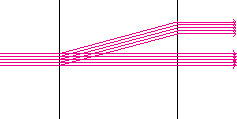
\includegraphics[width=\textwidth]{img/dvp}
    % \caption{Caption here}
    % \label{fig:figure1}
  \end{figure}	
\end{column}
\end{columns}

\end{frame}

\begin{frame}[t]
  \frametitle{Некоторые понятия теории физической оптики}
  \framesubtitle{Постоянная Верде}
 $V$ -- постоянная Верде -- скалярная физическая величина, характеризующая вращение плоскости поляризации света, распространяющегося вдоль линий магнитного поля, в которое помещено вещество.
\begin{equation}
	V=\frac{1}{\Theta}\int\limits_{0}^{L}B(x)dx
\end{equation}
где $\Theta$ -- угол, на который поворачивается плоскость поляризации.
$B(x)$ -- поле внутри образца длиной $L$.
\end{frame} 

\subsection{Цели и актуальность}
\begin{frame}[t]
  \frametitle{Цель и актуальность}
 \textbf{Цель}

  Изучение эффекта вращения плоскости поляризации на примере действия магнитного поля на теллуритные стекла; определение для каждого образца постоянной Верде.

\textbf{Актуальность}

    Эффект вращения плоскости поляризации света используется в:

  \begin{enumerate}
	 \item исследовании механических напряжений в прозрачных телах;
	\item компенсации термонаведенных эффектов, возникающих из-за нагрева оптических элементов;
	\item медицине (химико-фармацевтическом анализе);
  \end{enumerate}
\end{frame}

\begin{frame}[t]
  \frametitle{Вращатель Фарадея}
  \framesubtitle{Вращение плоскости поляризации}
  % \textbf{Изолятор/Вращатель Фарадея} -- образец из оптически неактивного вещества, помещённый в постоянное магнитное полею. 
  % Эффект Фарадея (1845г) -- вращение плоскости поляризации при прохождении пучка света через оптически неактивное вещество под действием магнитного поля.

  \begin{figure}[tb]
    \centering
    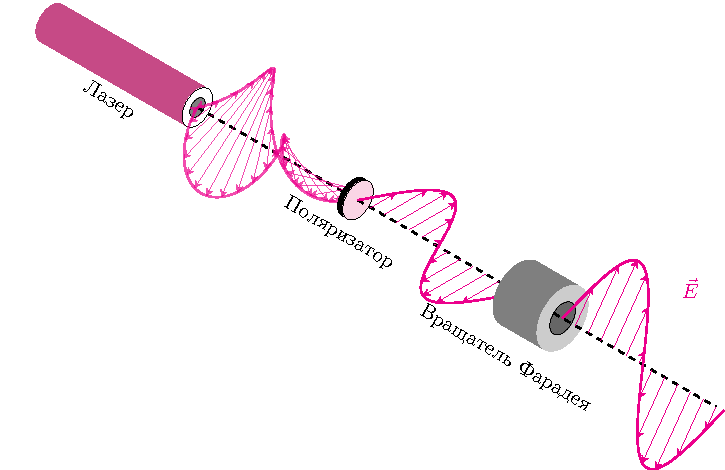
\includegraphics[width=\textwidth]{img/polarizing}
    % \caption{Caption here}
    % \label{fig:figure1}
  \end{figure}
\end{frame}


\section{Эксперимент}
\subsection{Схема установки}
\begin{frame}
\frametitle{Принципиальная схема установки}
\centering
\begin{tikzpicture}[
    media/.style={font={\footnotesize\sffamily}},
    wave/.style={
        decorate,decoration={snake,post length=1.4mm,amplitude=2mm,
        segment length=1mm},thick},
    interface/.style={
        % The border decoration is a path replacing decorator. 
        % For the interface style we want to draw the original path.
        % The postaction option is therefore used to ensure that the
        % border decoration is drawn *after* the original path.
        postaction={draw,decorate,decoration={border,angle=-45,
                    amplitude=0.3cm,segment length=1.3mm}}},
    ]

    % Round rectangle
    \fill[gray!10,rounded corners] (0,-1) rectangle ++(10,1);

    \begin{scope}[xshift=0cm]
	    \draw (0,0.5) rectangle node[above, yshift=1em] {LAS} ++(1,0.5);
	    \draw (0.5,0.5) -- (0.5,0);
	    \draw[blue,line width=.5pt,interface] (0,0) -- ++(1,0);    
    \end{scope}

    \draw[magenta, line width=2pt] (1,0.75) -- ++ (1,0);  
    \draw [red,  line width=1pt] (1.5,0.75) circle (4pt);
    \draw [->,red, line width=1pt] (1.5,0.5) -- ++ (0,0.6);
    \draw [->,red, line width=1pt] (3,0.5) -- ++ (0,0.6);
    \draw[magenta, line width=1pt] (2.5,0.75) -- ++ (2,0);  
    \draw[magenta, line width=1pt] (5.5,0.75) -- ++ (1.5,0);  
    \draw[magenta, line width=0.5pt] (7.5,0.75) -- ++ (1.5,0);  

    \begin{scope}[xshift=2cm]
    	\xdef\len{0.5cm}
	    \draw (0,0.5) rectangle node[above, yshift=1em] {POL} ++(\len,0.5);
	    \draw (\len/2,0.5) -- (\len/2,0);
	    \draw[blue,line width=.5pt,interface] (0,0) -- ++(\len,0);    
    \end{scope}    

    \begin{scope}[xshift=4.5cm]
	    \draw (0,0.5) rectangle node[above, yshift=1em] {F.J.} ++(1,0.5);
	    \draw (0.5,0.5) -- (0.5,0);
	    \draw[blue,line width=.5pt,interface] (0,0) -- ++(1,0);    
    \end{scope}  

    \begin{scope}[xshift=7cm]
    	\xdef\len{0.5cm}
	    \draw (0,0.5) rectangle node[above, yshift=1em] {FILTER} ++(\len,0.5);
	    \draw (\len/2,0.5) -- (\len/2,0);
	    \draw[blue,line width=.5pt,interface] (0,0) -- ++(\len,0);    
    \end{scope} 

    \begin{scope}[xshift=9cm]
    	\xdef\len{1cm}
	    \draw (0,0.5) rectangle node[above, yshift=1em] {CAM} ++(\len,0.5);
	    \draw (\len/2,0.5) -- (\len/2,0);
	    \draw[blue,line width=.5pt,interface] (0,0) -- ++(\len,0);    
    \end{scope}       
    % \draw[-latex,thick](5.25,0.5)node[right]{}
         % ..controls +(180:.2cm) and +(up:0.25cm) .. (5,0);
\end{tikzpicture}	
\end{frame}

\subsection{Распределение магнитного поля}
\begin{frame}[t]\frametitle{Распределение поля $B$ в постоянном магните}
\centering
  \begin{tikzpicture}
  \begin{axis}[
    xlabel={$l$, mm},
    ylabel={$B$, T}]
  \addplot[smooth] table [x=l, y=10t, col sep=tab] {data/b_x.csv}; 
  \end{axis}
  \end{tikzpicture}    
\end{frame}

\subsection{Результаты эксперимента}
\begin{frame}[t]\frametitle{Результаты эксперимента}
\centering
  \begin{tikzpicture}[scale=0.95]
  \begin{axis}[
    xlabel={$\lambda$, nm},
    ylabel={$V$},
    domain=400:2000, 
    legend pos = north west,
    ]
  \legend{}
  \xdef\A{10660}
  \xdef\B{0.6846}
  \xdef\C{0.8858}
  \addplot[magenta]{1/x*(\A+\B/(x^2-\C^2))};    
    \addplot[color=magenta, draw=none,mark=x] coordinates {
    (531,22.8)
    (658,13.24)
    (1064,9.36)
  };
  \xdef\A{13700}
  \xdef\B{0.9157}
  \xdef\C{0.4347}
  \addplot[blue]{1/x*(\A+\B/(x^2-\C^2))};    
    \addplot[color=blue, draw=none,mark=x] coordinates {
    (531,31.74)
    (658,15.25)
    (1064,5.48)
  };  
  \xdef\A{11400}
  \xdef\B{0.8769}
  \xdef\C{0.159}
  \addplot[black]{1/x*(\A+\B/(x^2-\C^2))};    
    \addplot[color=black, draw=none,mark=x] coordinates {
    (531,24.3)
    (658,14.05)
    (1064,10.36)
  };  
  \xdef\A{13910}
  \xdef\B{0.5898}
  \xdef\C{0.1144}
  \addplot[green]{1/x*(\A+\B/(x^2-\C^2))};    
    \addplot[color=green, draw=none,mark=x] coordinates {
    (531,29.58)
    (658,17.12)
    (1064,12.79)
  };   
  \xdef\A{14670}
  \xdef\B{0.2769}
  \xdef\C{0.1981}
  \addplot[magenta!40!blue]{1/x*(\A+\B/(x^2-\C^2))};    
    \addplot[color=magenta!40!blue, draw=none,mark=x] coordinates {
    (531,30.77)
    (658,19.68)
    (1064,11.69)
  };        
  \end{axis}
  \end{tikzpicture}    
\end{frame}

\section{Выводы}
\begin{frame}
  % \transdissolve[duration=0.2]
  \frametitle{Заключение}
  	В ходе этого эксперимента мы 
  	\begin{enumerate}
  	 	\item ознакомились с эффектом Фарадея;
  	 	\item определили для магнитоактивных материалов постоянную Верде; 
  	 	\item провели серию экспериментов с образцами магнитоактивных материалов;
  	 \end{enumerate} 
  	 
    
\end{frame}

\end{document}